% !TeX spellcheck = de_DE
\documentclass{uebung_cs}
\usepackage{algo221}
\uebung{8}{}{}
\blattname{Übungen zu Woche 8: Hartnäckigkeit II}

\usepackage[ruled]{algorithm2e}
%\usepackage{circuitikz}

%%%%%%%%%%%%%%%%%%%%%%%%%%%%%%%%%%%%%%%%%%%%%%%%%%%%%%%%%%%%%%%%%%%%%%%%%%%%
\begin{document}

Das Übungsblatt enthält alle empfohlenen Lernaktivitäten für die aktuelle Woche.

\begin{itemize}
\item \textbf{Heimarbeit bis Montag 17:00.}
    \begin{itemize}
    \item 
    Schau die Videos an und lies die Buchkapitel.
    \item Bearbeite die \emoji{seedling}-Aufgabe in \href{https://moodle.studiumdigitale.uni-frankfurt.de/moodle/course/view.php?id=2241}{Moodle}. (Feste Abgabefrist!)
    \item Lese den Aufgabentext aller Übungsaufgaben.
    \end{itemize}
\item \textbf{Heimarbeit.} Bearbeite die Übungsaufgaben soweit möglich. Probier zumindest alle mal!
\item \textbf{Dienstag/Donnerstag.}
\begin{itemize}
    \item \textbf{8:00--8:15.} Besprechung im Hörsaal.
    \item \textbf{8:15--9:15.} Bearbeite jetzt die Übungen, die du noch nicht lösen konntest. Sprich mit anderen Studis! Frag das Vorlesungsteam um Hilfe!
    \item \textbf{9:15--9:45.} Lösungsspaziergang zu den Aufgaben für heute.
\end{itemize}

\item \textbf{Heimarbeit bis Freitag, den 10.12., 17:00.} Gib deine Lösungen zu der \emoji{star}-Aufgabe von diesem Übungsblatt in \href{https://moodle.studiumdigitale.uni-frankfurt.de/moodle/course/view.php?id=2241}{Moodle} ab. (Feste Abgabefrist!)
\end{itemize}

\section*{Dienstag}

\begin{aufgabe}[k-COLOR]\
	% https://courses.engr.illinois.edu/cs374/fa2021/A/labs/lab13.pdf - Exercise 1
	\begin{quote}
		$k$-\textsc{Color}:\\
		Gegeben sei ein ungerichteter Graph $G = (V,E)$. Können alle Knoten $v \in V$ mit $k$ Farben so gefärbt werden, dass jede Kante inzident zu zwei Knoten unterschiedlicher Farbe ist?
	\end{quote}
	\begin{enumerate}
		\item Beschreibe eine polynomielle Reduktion von \textsc{3Color} zu \textsc{4Color}.
		\item Zeige, dass $k$-\textsc{Color} für jedes $k \geq 3$ $\NP$-hart ist.
	\end{enumerate}
\end{aufgabe}

\begin{aufgabe}[$\NP$-Härte]\
	% https://courses.engr.illinois.edu/cs374/fa2021/A/labs/lab13.pdf - Exercise 2
	Zeige, dass die folgenden Probleme $\NP$-hart sind.
	\begin{enumerate}
		\item Gegeben sei ein ungerichteter Graph $G$. Enthält $G$ einen einfachen Pfad, der alle außer 247 Knoten besucht?
		\item Gegeben sei ein ungerichteter Graph $G$. Enthält $G$ einen Spannbaum, in dem jeder Knoten einen Grad von höchstens $198$ hat?
		\item Gegeben sei ein ungerichteter Graph $G$. Enthält $G$ einen Spannbaum mit höchstens $350$ Blättern?
	\end{enumerate}
\end{aufgabe}

\section*{Donnerstag}

\begin{aufgabe}[Ressourcenmanagement]
	% KT - Exercise 8.4
	Ein Unternehmen verwaltet High-Performance Echtzeitsysteme mit asynchronen Prozessen, die auf gemeinsame Ressourcen zugreifen müssen. Das System hat eine Menge von $n$ Prozessen und eine Menge von $m$ Ressourcen. 
	Zu jedem Zeitpunkt spezifiziert ein Prozess eine Menge an Ressourcen, die er benutzen möchte. Jede Ressource kann gleichzeitig von mehreren Prozessoren angefragt werden, aber es kann zu jedem Zeitpunkt nur \emph{genau} ein Prozess auf die Ressource zugreifen. 
	
	Deine Aufgabe ist es, die Ressourcen an die Prozesse zu verteilen. Wenn ein Prozess alle benötigten Ressourcen zugeteilt bekommt, ist er \textit{aktiv}, ansonsten ist er \textit{blockiert}. Eine effiziente Zuweisung der Ressourcen sorgt dafür, dass möglichst viele Prozesse \textit{aktiv} sind, was sich als das Problem \textsc{RessourcenReservieren} ausdrücken lässt.
	 \begin{quote}
	 \textsc{RessourcenReservieren}:\\
	 Es sei eine Menge von $n$ Prozessen, eine Menge von $m$ Ressourcen und eine Zahl $k$ gegeben. Ist es möglich, die Ressourcen den Prozessen so zuzuweisen, dass mindestens $k$ Prozesse \textit{aktiv} sind?
	 \end{quote}
	 
	Gib für jedes Problem auf der folgenden Liste entweder einen Polynomialzeit-Algorithmus an oder zeige, dass das Problem \NP-vollständig ist.
	 \begin{enumerate}
	 	\item \textsc{RessourcenReservieren}.
	 	\item \textsc{RessourcenReservieren} mit dem Spezialfall $k=2$.
	 	\item \textsc{RessourcenReservieren} mit zwei Typen von Ressourcen. Hierbei sind die Ressourcen: Mensch und Maschine. Jeder Prozess benötigt höchstens eine Ressource von jedem Typ. (Anders ausgedrückt braucht jeder Prozess einen bestimmten Menschen und eine bestimmte Maschine.)
	 	\item \textsc{RessourcenReservieren} mit dem Spezialfall, dass jede Ressource von maximal zwei Prozessen angefragt wird.	 	
	 \end{enumerate}
\end{aufgabe}

\begin{aufgabe}[Zweifärbung]
	% https://courses.engr.illinois.edu/cs374/fa2021/A/labs/lab13bis.pdf - Exercise 3
	Eine Zweifärbung eines ungerichteten Graphen $G = (V,E)$ weist jedem Knoten $v \in V$ eine Menge von zwei unterschiedlichen Farben $\{f_1,f_2\} \in F$ zu. Es gibt zwei Arten der Zweifärbung:
	\begin{itemize}
		\item In einer \textit{schwachen} Zweifärbung (siehe Abbildung~\ref{schwach}) müssen die zu jeder Kante inzidenten Knoten verschiedene Farbmengen besitzen. Die beiden Mengen dürfen sich aber eine Farbe teilen.
		\item In einer \textit{starken} Zweifärbung (siehe Abbildung~\ref{stark}) müssen die zu jeder Kante inzidenten Knoten komplett unterschiedliche Farbmengen haben. Das heißt, eine Kante ist inzident zu $4$ Farben.
	\end{itemize}
	Jede starke Zweifärbung ist auch eine schwache Zweifärbung.
	\begin{enumerate}
		\item Zeige, dass es $\NP$-hart ist, für einen gegebenen ungerichteten Graphen $G$ die minimale Anzahl an Farben in einer schwachen Zweifärbung zu finden.
		\item Zeige, dass es $\NP$-hart ist, für einen gegebenen ungerichteten Graphen $G$ die minimale Anzahl an Farben in einer starken Zweifärbung zu finden.
	\end{enumerate}
	\begin{figure}[ht]
	    \begin{minipage}{0.5\linewidth}
	        \centering
	        		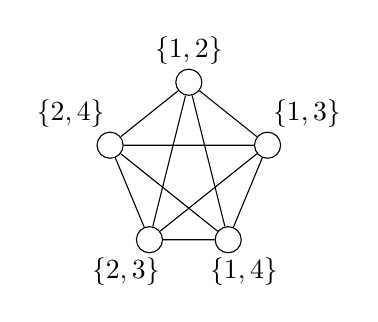
\begin{tikzpicture}
                    \node[draw,circle] (a) at (0,0.2) {};
                    \node[] (label_1) at (-0.5,0.6) {$\{2,4\}$};
                    \node[draw,circle] (b) at (1,1) {};
                    \node[] (label_2) at (1,1.4) {$\{1,2\}$};
                    \node[draw,circle] (c) at (2,0.2) {};
                    \node[] (label_3) at (2.5,0.6) {$\{1,3\}$};
                    \node[draw,circle] (d) at (1.5,-1) {};
                    \node[] (label_4) at (1.7,-1.4) {$\{1,4\}$};
                    \node[draw,circle] (e) at (0.5,-1) {};
                    \node[] (label_5) at (0.2,-1.4) {$\{2,3\}$};
            
                    \draw  (a) -- (b)
                           (a) -- (c)
                           (a) -- (d)
                           (a) -- (e)
                           (b) -- (c)
                           (b) -- (d)
                           (b) -- (e)
                           (c) -- (d)
                           (c) -- (e)
                           (d) -- (e);
                \end{tikzpicture}
                \caption{Eine schwache Zweifärbung.}\label{schwach}
	    \end{minipage}
	    \begin{minipage}{0.5\linewidth}
	        \centering
	            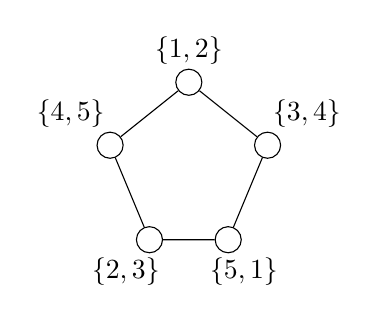
\begin{tikzpicture}
                    \node[draw,circle] (a) at (0,0.2) {};
                    \node[] (label_1) at (-0.5,0.6) {$\{4,5\}$};
                    \node[draw,circle] (b) at (1,1) {};
                    \node[] (label_2) at (1,1.4) {$\{1,2\}$};
                    \node[draw,circle] (c) at (2,0.2) {};
                    \node[] (label_3) at (2.5,0.6) {$\{3,4\}$};
                    \node[draw,circle] (d) at (1.5,-1) {};
                    \node[] (label_4) at (1.7,-1.4) {$\{5,1\}$};
                    \node[draw,circle] (e) at (0.5,-1) {};
                    \node[] (label_5) at (0.2,-1.4) {$\{2,3\}$};
            
                    \draw  (a) -- (b)
                           (b) -- (c)
                           (c) -- (d)
                           (d) -- (e)
                           (e) -- (a);
                \end{tikzpicture}
                \caption{Eine starke Zweifärbung.}\label{stark}
	    \end{minipage}
	\end{figure}
\end{aufgabe}

%\begin{aufgabe}[Clique]
	% Algorithms and Data Structures 2 - NP.pdf
%	Für einen ungerichteten Graphen $G = (V,E)$  ist eine \textit{Clique} eine Teilmenge $V' \subseteq V$ der Knotenmenge, sodass alle Knoten in $V'$ benachbart sind, also wenn zwischen jedem Knotenpaar $v,w \in V'$ mit $v \neq w$ eine Kante $(v,w) \in E$ existiert. Ein Graph $G$ hat eine $k$-\textit{Clique}, wenn $|V'| = k$ gilt. Das Entscheidungsproblem \textsc{Clique} ist wie folgt definiert:
%	\begin{quote}
%		\textsc{Clique}:\\
%		\textit{Input:} Ein ungerichteter Graph $G = (V,E)$ und ein $k \in \mathbb{N}_0$.\\
%		\textit{Output:} \glqq JA\grqq{}, wenn $G$ eine $k$-\textit{Clique} besitzt, sonst \glqq NEIN\grqq{}.
%	\end{quote}
%	\begin{enumerate}
%		\item Zeige, dass \textsc{Clique} $\in \NP$.
%		\item Zeige, dass \textsc{Clique} \NP-vollständig ist, indem du \textsc{IndependentSet} auf \textsc{Clique} reduzierst.
%	\end{enumerate}
%\end{aufgabe}

\newpage

\section*{Sternaufgabe}

\begin{aufgabe}[\emoji{star}: Vorsichtige Färbung]
	% Ericksen, Chapter 12, Exercise 24
	Eine $5$-\textsc{Färbung} eines Graphen $G = (V,E)$ weist jedem Knoten $v \in V$ eine \glqq Farbe\grqq{} aus der Menge $\{0,1,2,3,4\}$ zu, sodass $u,v \in V$ für jede Kante $(u,v) \in E$ unterschiedliche \glqq Farben\grqq{} haben. Eine $5$-\textsc{Färbung} ist \textit{vorsichtig}, wenn die Farben adjazenter Knoten sich um mindestens $(1 \mod 5)$ unterscheiden. Zeige, dass das Entscheidungsproblem, ob ein gegebener Graph eine vorsichtige $5$-\textsc{Färbung} besitzt, $\NP$-hart ist.
	
	\textit{Tipp: Benutze für die Reduktion das normale $5$-\textsc{Färbung}-Problem}.
	
	\begin{figure}[ht]
	\begin{center}
		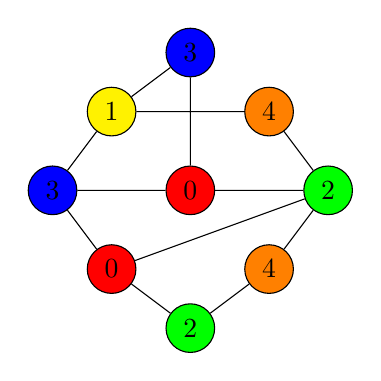
\begin{tikzpicture}
            \node[draw,circle,fill=red] (a) at (0,0) {$0$};
            \node[draw,circle,fill=blue] (b) at (0,1.75) {$3$};
            \node[draw,circle,fill=orange] (c) at (1,1) {$4$};
            \node[draw,circle,fill=green] (d) at (1.75,0) {$2$};
            \node[draw,circle,fill=orange] (e) at (1,-1) {$4$};
            \node[draw,circle,fill=green] (f) at (0,-1.75) {$2$};
            \node[draw,circle,fill=red] (g) at (-1,-1) {$0$};
            \node[draw,circle,fill=blue] (h) at (-1.75,0) {$3$};
            \node[draw,circle,fill=yellow] (i) at (-1,1) {$1$};
            
            \draw  (a) -- (b)
                   (a) -- (d)
                   (a) -- (h)
                   (b) -- (i)
                   (i) -- (c)
                   (d) -- (g)
                   (c) -- (d)
                   (d) -- (e)
                   (e) -- (f)
                   (f) -- (g)
                   (g) -- (h)
                   (h) -- (i);
        \end{tikzpicture}
        \caption{Ein Beispiel für eine vorsichtige $5$-\textsc{Färbung}.}
	\end{center}
	\end{figure}
\end{aufgabe}

\end{document}
